\documentclass[tikz,border=8pt]{standalone}
\usepackage{lmodern}
\usetikzlibrary{arrows.meta,calc,patterns,decorations.pathreplacing}
\definecolor{ink}{HTML}{183B4E}
\definecolor{teal}{HTML}{168C8C}
\definecolor{gold}{HTML}{D9982F}
\definecolor{violet}{HTML}{7B61A8}
\definecolor{softblue}{HTML}{EAF4F6}
\definecolor{softgold}{HTML}{FFF4D8}
\begin{document}
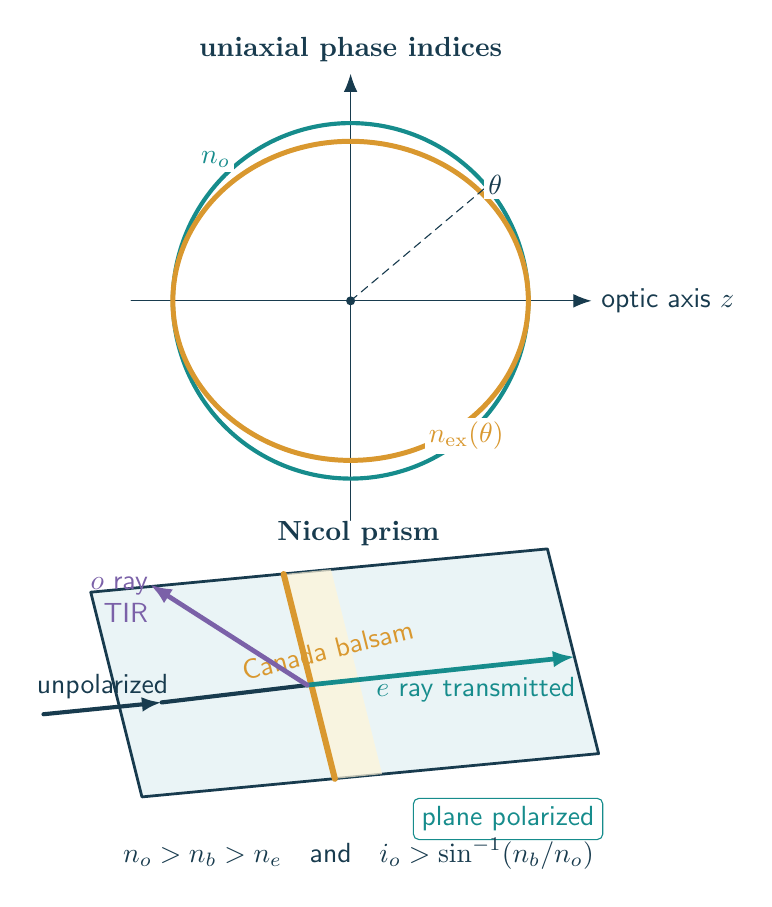
\begin{tikzpicture}[>=Latex,line cap=round,line join=round,font=\sffamily]
  % Index surfaces, generated from n_ex(theta).
  \begin{scope}[shift={(3.9,6.15)},scale=1.36]
    \node[ink,font=\bfseries] at (0,2.35) {uniaxial phase indices};
    \draw[ink,-{Latex[length=2.3mm]}] (-2.05,0)--(2.25,0) node[right] {optic axis $z$};
    \draw[ink,-{Latex[length=2.3mm]}] (0,-2.05)--(0,2.12);
    \draw[teal,line width=1.5pt]
      plot[domain=0:360,samples=241,variable=\t]
      ({1.66*cos(\t)},{1.66*sin(\t)});
    \draw[gold,line width=1.8pt]
      plot[domain=0:360,samples=241,variable=\t]
      ({(1.66*1.49/sqrt(1.49^2*cos(\t)^2+1.66^2*sin(\t)^2))*cos(\t)},
       {(1.66*1.49/sqrt(1.49^2*cos(\t)^2+1.66^2*sin(\t)^2))*sin(\t)});
    \draw[ink,densely dashed] (0,0)--({1.78*cos(40)},{1.78*sin(40)});
    \node[ink,fill=white,inner sep=1.5pt] at (1.35,1.08) {$\theta$};
    \node[teal,fill=white,inner sep=1.5pt] at (-1.26,1.32) {$n_o$};
    \node[gold,fill=white,inner sep=1.5pt] at (1.08,-1.26) {$n_{\rm ex}(\theta)$};
    \fill[ink] (0,0) circle (1.2pt);
  \end{scope}

  % Nicol prism schematic.
  \begin{scope}[shift={(1.25,-0.15)}]
    \node[ink,font=\bfseries] at (2.75,3.35) {Nicol prism};
    \path[fill=softblue,draw=ink,line width=1pt]
      (0,0)--(5.8,0.55)--(5.15,3.15)--(-0.65,2.60)--cycle;
    \path[fill=softgold,opacity=.7]
      (2.45,0.23)--(3.05,0.29)--(2.40,2.89)--(1.80,2.83)--cycle;
    \draw[gold,line width=2.2pt] (2.45,0.23)--(1.80,2.83);
    \node[gold,rotate=14,anchor=south] at (2.42,1.63) {Canada balsam};

    \coordinate (A) at (-1.25,1.05);
    \coordinate (B) at (0.25,1.20);
    \coordinate (C) at (2.10,1.42);
    \coordinate (E) at (5.50,1.78);
    \coordinate (Q) at (0.10,2.70);
    \draw[ink,line width=1.5pt,-{Latex[length=2.5mm]}] (A)--(B);
    \draw[ink,line width=1.5pt] (B)--(C);
    \draw[teal,line width=1.7pt,-{Latex[length=2.8mm]}] (C)--(E);
    \draw[violet,line width=1.7pt,-{Latex[length=2.8mm]}] (C)--(Q);
    \node[ink,above] at ($(A)!0.5!(B)$) {unpolarized};
    \node[teal,below] at ($(C)!0.63!(E)$) {$e$ ray transmitted};
    \node[violet,left,align=right] at (0.20,2.50) {$o$ ray\\TIR};
    \node[teal,draw=teal,rounded corners=2pt,fill=white,inner sep=3pt]
      at (4.65,-0.28) {plane polarized};
    \node[text=ink,align=center] at (2.75,-0.72)
      {$n_o>n_b>n_e$\quad and\quad $i_o>\sin^{-1}(n_b/n_o)$};
  \end{scope}
\end{tikzpicture}
\end{document}
